\chapter{Ausgangssituation und Zielsetzung}

\section{Ausgangssituation}
Die HTBLA-Leonding ist eine BHS im Raum Oberösterreich, welche für ihre gute Ausbildung und interessanten Projekte im Bereich der Informationstechnologie bekannt ist.

\section{Beschreibung des Problembereichs}
In den Klassenräumen fehlt es oft an Sauerstoff, manchmal ist auch die Temperatur nicht adäquat. Dieseh kann eine Reihe von unerwünschten Symptomen hervorrufen, wie zum Beispiel: 

\begin{itemize}
    \item Kopfschmerzen
    \item Ermüdung
    \item Schwindel
    \item Übelkeit
    \item mehr Probleme mit Asthma und Allergien
\end{itemize}

Die oben gennannten Symptome sind in einer Umgebung wie der Schule unbedingt zu vermeiden, da es ansonsten zu einem Konzentrationsverlust der Schüler führt.

Um zusätzlich eine Regelung der Heizung vornehmen zu können sind weitere Informationen der einzelnen Klassenräume, wie die Temperatur, notwendig. Weiters wird es rund um die Uhr ermöglicht,  geöffnete Fenster zu lokalisieren und mit dieser Information Schäden an der Schule zu verhindern.

\section{Aufgabenstellung}
%todo
drei Ebenen
nodes senden Nachrichten
ota
systemarchitektur
dann einzelne Komponente

\begin{figure}[H]
    \centering
    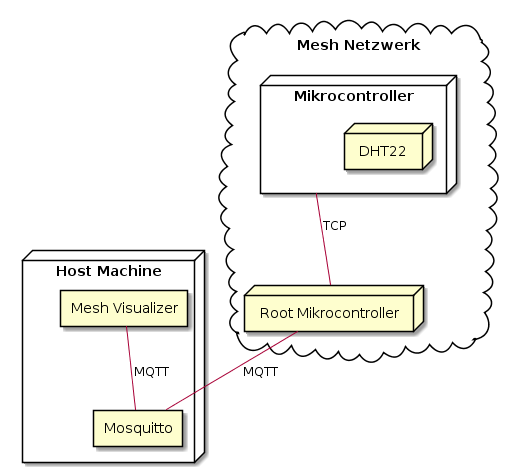
\includegraphics[scale=0.8]{diagrams/deployment.png}
    \caption{Systemarchitektur (Quelle: Eigene Darstellung)}
    \label{abb:deployment}
\end{figure}

Um die Sensoren in der Schule platzieren zu können, ist es erforderlich, zuerst eine Infrastruktur für die Auswertung der Sensoren zu gestalten.

\section{Zielbestimmung}
Unterricht findet in einer Lernumgebung statt
Schüler lernen

Die Knoten eines Mesh-Netzwerks können gegenseitig Nachrichten versenden und reagieren automatisch auf ausfallende Knoten.